\section{Introduction}
\label{sec:introduction}
% Motivation.
Understanding the moving trajectories of millions of vehicles in a city offers valuable insights into urban mobility, enabling applications such as usage-based electronic toll collection, accurate traffic analysis, intelligent traffic light control, and retrospective urban planning analysis.
% Related work.
Current trajectory reconstruction methods rely on in-vehicle devices (e.g., GPS) for partial knowledge, and roadway monitoring with flow sensors (e.g., loop detectors, piezoelectric sensors, infrared sensors) for capturing traffic flows.

% Their work and contributions.
This research explores the use of traffic cameras as a sensing network to accurately recreate citywide vehicle trajectory.
The traffic camera network offers advantages over existing alternatives, including: (i) Traffic cameras are widely available and cost-effective for urban deployment; (ii) They provide high coverage for sensing and monitoring vehicle trajectories; (iii) Advanced image analysis techniques can extract vehicle identifiers, enabling trajectories recovery with higher accuracy.
Vetrac was experimented on using real-world data collected from one full day of one of China's urban road networks, which covers $66 km^2$.
\Cref{fig:china-road-representation} represents the road network, where white dots present rear-view cameras, while red dots present front-view cameras.
Each camera records the following information: camera metadata, snapshot, entering time, exit time, and lane directions.
Overall, seven million snapshots were collected, and 1,247,835 vehicle trajectories have been reconstructed.

\begin{figure}
\centering
  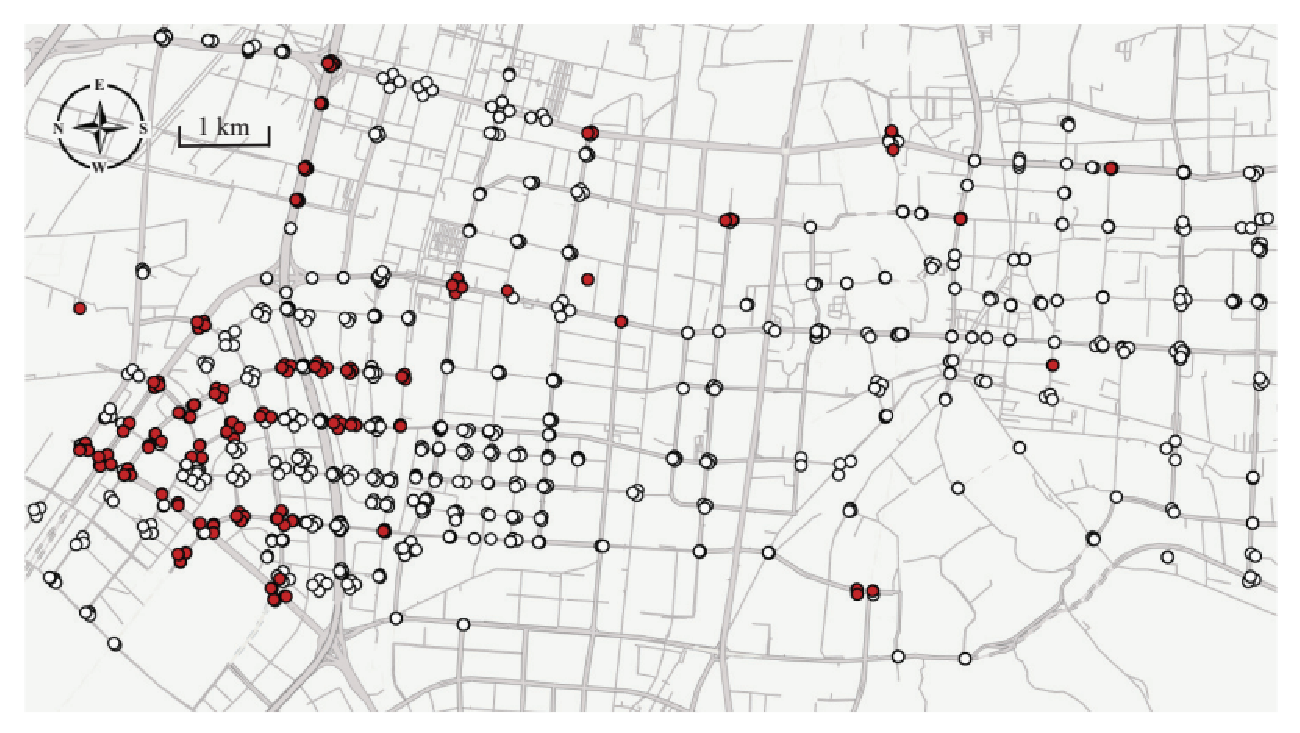
\includegraphics[width=0.9\linewidth]{figures/china-road-network.eps}
  \caption{China's road network \cite{tong2021large}}
  \label{fig:china-road-representation}
  %\vspace{-5mm}
\end{figure}

The structure of the rest of the paper is as follows:
\Cref{sec:sensing-challenges} presents the challenges that face the current sensing techniques.
In \Cref{sec:related-work}, we present the related work, while in \Cref{sec:scheme}, we present the proposed scheme.
Moreover, the evaluations are presented in \Cref{sec:discussion_evaluations}.
Finally, the work is concluded in \Cref{sec:conclusions}.
